\documentclass[../thesis.tex]{subfiles}

\begin{document}

%\chapter{Classification and Regression Trees}
\chapter{Predictive Analytics}
\section{Introduction}
%Classification and regression trees (CART) are a type of predictive algorithm used to group similar attributes together.
Predictive analytics uses statistics and modelling techniques to make predictions about future events \cite{Kumar2018}. By analysing current and historical data, it allows businesses to become more proactive by looking forward at anticipating trends or behaviour, with the potential to save time, cost and resources. This thesis examines the use of classification and regression (CART) trees to identify similar groupings of patient attributes.%\hl{TBD - one or two} predictive algorithms. The first method discussed is the application of Classification and regression trees (CART) to group similar attributes together. 

As discussed within Chapter \ref{chp:LiteratureReview}, predictive and forecasting techniques were the most common research aim within literature. However, the research tended to use more traditional OR/MS methods to achieve this, e.g., Simulation and Markov Chains. This chapter aims to address the research question 1, `How do the clinical and demographical attributed of elderly and frail patients effect their length of stay within hospital', by using less traditional OR/MS methods. This chapter is structured as follows:
%Predictive analytics



\section{Prediction Techniques}
A classification and regression tree (CART) is a predictive model which determine how variables can predict an outcome. A decision tree is produced as a visual aid, where each split in the ‘branch’ is a split in a predictor variable and each node (leaf) contains a prediction for the outcome variable. A classification tree is used when the dependent variable is categorical and regressions trees are used when the dependent variable is continuous. We aim to predict the LOS of a patient within hospital using the demographical and clinical attributes. Whilst LOS is a continuous measure, we can discretize this into categories to increase the suitability of the model. 

To determine suitability of variables, we will be used four traditional scoring measures:
\begin{align}
R^{2} = \\
    \text{Accuracy} = & \frac{\text{True positive}+\text{True negative}}{\text{Total number of observations}}\\
    \text{Precision} = & \frac{\text{True positive}}{\text{True positive}+\text{True negative}}\\
    \text{Recall} = & \frac{\text{True positive}}{\text{True positive}+\text{False negative}}
\end{align}
There are ten different factors within the data which could have an effect LOS, which will be used in the building of the tree:
\begin{multicols}{2}
\begin{itemize}
\item Admission Method
    \item Admission Source
    \item Age
    \item Day of admission
    \item Diagnosis/ICD10
    \item Frailty Score
    \item Hospital
    \item Month of admission
    \item Scan information
    \item Specialty
\end{itemize}
\end{multicols}
To determine the suitability of using each variable we can evaluate using linear and logistic regressions.
\section{Analysing prediction variables individually}
Within our data set, there are two different types, continuous and categorical. Age and frailty score are the only two variables which are continuous, however as discussed in Chapter \ref{chp:Data}, can be converted into categorical.
As there are $>$3000 data points, can assume normality and run linear regressions to evaluate relationships (\hl{REF}).
% The frailty score was also split into three groups to determine if this improves prediction: 
% \begin{itemize}
%     \item Frailty = 0 (120,779 $\approx$ 73.16\%)
%     \item 0 $<$ Frailty $\leq$ 2.2 (27,014 $\approx$ 16.36\%)
%     \item Frailty $>$ 2.2 (17305 $\approx$ 10.48\%)
% \end{itemize}

\subsection{Linear Regression}
Linear regression is used to predict the value of the dependent variable based on the value of independent variables. The R$^2$ value is a goodness of fit measure, which will determine how much variation of a dependent variable is explained by the independent variable.
The linear regression model can be denoted as:
\begin{equation}
    y  = \beta_{0} + \beta_{1}x + \epsilon
\end{equation}
 By using ordinary least squares (OLS), we can estimate the regression R$^{2}$ result for each of the variables included within the data (Table \ref{Tab:ContinuousLOS-Lin}). Additionally, the adjusted R$^{2}$ value is calculated, which takes into account the number of variables that is included within the model.

\begin{table}[h!]
\centering\scalebox{1}{
\begin{tabular}{ccc}
\toprule
\textbf{Variable} & \textbf{R$^2$ Value}&\textbf{Adjusted R$^2$ Value} \\ \midrule 
Age & 0.204 & 0.204 \\
Age Group &  0.051 & 0.051 \\
Admission Method & 0.282 & 0.282  \\
Admission Source & 0.195 & 0.195 \\
Day of Admission & 0.002& 0.002\\
Diagnosis & 0.273 & 0.261\\
Frailty Score & 0.043 & 0.043\\
Frailty Group & 0.028& 0.028\\
Hospital & 0.182 & 0.181 \\
ICD10 - First Letter & 0.092& 0.092\\
No. of Scans & 0.030 & 0.030\\
Scan Y/N & 0.025 & 0.025 \\
Month of Admission & 0.000& 0.000\\
Specialty & 0.288 & 0.288\\\bottomrule
\end{tabular}}
\caption{Linear Regression Result}
\label{Tab:ContinuousLOS-Lin}
\end{table}



There are two types of data, continuous and categorical. The Specialty of a patient accounts for the most...

\underline{Continuous Example}
\begin{lstlisting}[style=pystyle]
>>> import pandas as pd
>>> import statsmodels.api as sm
>>> x = pd.DataFrame(df['Age_on_Arrival']) 
>>> y = pd.DataFrame(df['LOS'])
>>> model = sm.OLS(y, x).fit()
>>> print(model.summary())
\end{lstlisting}


The R$^2$ value for age is 0.05. This means 5\% of the LOS variation is explained by Age. The model can be denoted by: 
\begin{equation}
    Y = 0.375x - 22.635
\end{equation}
Therefore, for each 1 year increment in age, the LOS will increase by 0.375 days.
\underline{Categorical Example}\\
Similarly, we can perform linear regression on categorical variables. In order to achieve this one-hot coding must be used.
\begin{lstlisting}[style=pystyle]
>>> import pandas as pd
>>> import statsmodels.api as sm
>>> x = df['Specialty']
>>> x = pd.get_dummies(data=x)
>>> y = pd.DataFrame(df['LOS'])
>>> model = sm.OLS(y, x).fit()
>>> print(model.summary())
\end{lstlisting}
There is a total of 29 different specialties within the data. Equation \ref{eq:LinCat} denoted the resulting model produced from the above code. For the specialty admitted under, the equivalent $x_i$ will be given a value of 1, and the remaining $x_i$ values are given a 0. For example if a patient attends Accident \& Emergency, $x_1$ =1 and $x_2 - x_29$ = 0 and therefore $Y=2.2673$ days.

\begin{multline}\label{eq:Lincat}
    Y = 2.2673x_1 + 14.9517x_2 +4.647x_3 +12.1101x_4 + 34.235x_5 +0.2616x_6 + 11.6161x_7+\\ 
    2.75x_8 +39.2603x_9 + 2.1382x_{10} +8.4519x_{11} + 3.7149x_{12} + 1.6536x_{13} + 0.7974x_{14} + \\
    11.6289x_{15} + 14.3725x_{16} + 0.6018x_{17} + 5.6131x_{18}+ 0.1307x_{19} + 0.0080x_{20} + 0.1128x_{21} + \\
    0.3548x_{22} + 13.6667x_{23} + 28.7732x_{24} + 7.7985x_{25} + 0x_{26} + 2.3333x_{27} + 6.6658x_{28} + 0.9932x_{29}
\end{multline}
where $x_{1}$ = Accident \& Emergency, $x_{2}$ = Anaesthetics, $x_{3}$ = Cardiology, $x_{4}$ = Care of the Elderly, $x_{5}$ = Community Medicine, $x_{6}$ = Dermatology, $x_{7}$ = Diabetes \& Endocrinology, $x_{8}$ = Ear Node \& Throat, $x_{9}$ = GP Other, $x_{10}$ = Gastroenterology, $x_{11}$ = General Medicine, $x_{12}$ = General Surgery, $x_{13}$ = Gynaecology, $x_{14}$ = Haematology, $x_{15}$ = Infectious Diseases, $x_{16}$ = Intermediate Care, $x_{17}$ = Maxillo-Facial, $x_{18}$ = Neurology, $x_{19}$ = Opthalmology, $x_{20}$ = Pain, $x_{21}$ = Plastic Surgery, $x_{22}$ = Radiology, $x_{23}$ = Radiotherapy \& Oncology, $x_{24}$ = Rehabilitation, $x_{25}$ = Respiratory, $x_{26}$ = Restorative Dentistry, $x_{27}$ = Rheumatology, $x_{28}$ = Trauma \& Orthopaedic ,$x_{29}$ = Urology.\\

\subsection{Grouped LOS - Logistic regression}\\
Logistic regressions were performed to determine the accuracy of the variables. The LOS was grouped into 0 days (i.e., discharged/transferred on same say as admission), and those patients who had a minimum of a one night stay. Similar to linear regression, we performed analysis on all variables (Table \ref{}).
\begin{equation}
    logit(p) = log(\frac{p}{(1-p)}) = \beta_0 + \beta_1 x_1 + ... + \beta_{k} x_{k}
\end{equation}

\begin{table}[h!]
\centering\scalebox{1}{
\begin{tabular}{cccc}
\toprule
\multirow{2}{*}{\textbf{Variable}} &  \multicolumn{3}{c}{\textbf{Logistic Regression}}  \\ %\cline{3-5}
&\textbf{Accuracy}& \textbf{Precision} & \textbf{Recall}\\ \midrule
Age  & 0.6037 &0.6259 & 0.6768\\
Age Group & 0.6037 & 0.6259 & 0.6768\\
Admission Method & 0.8764 &0.9137 & 0.8536  \\
Admission Source & 0.5829 & 0.5663 & 1.0 \\%\multicolumn{3}{c}{Too many variables}\\
Day of Admission & 0.5474 & 0.8343 & 0.8389\\
Diagnosis  & 0.8128 & 0.7967 & 0.8811 \\
Frailty Score  & 0.5860 & 0.7444& 0.3648\\
Frailty Group  & 0.5871 & 0.7451 & 0.3673\\
Hospital& 0.6171 & 0.5996 & 0.8933 \\
ICD10 - First Letter & 0.7554 & 0.7399 & 0.8494 \\
No. of Scans & 0.5445 & 0.5445 & 1.0\\
Scan Y/N & 0.8558 & 0.8558& 1.0\\
Month of Admission & 0.5445 & 0.5445& 1.0 \\
Specialty & 0.8008 & 0.8349 & 0.7905 \\\bottomrule
\end{tabular}}
\caption{Linear Regression and Logistic Regression Result}
\label{Tab:ContinuousLOS-Log}
\end{table}

\underline{Continuous Example}



\begin{lstlisting}[style = pystyle]
>>> import statsmodels.formula.api as smf
>>> from statsmodels.formula.api import logit
>>> model = smf.logit("LOSGroup ~ diagnosis", data = df)
>>> results = model.fit()
\end{lstlisting}
\subsection{Grouped LOS - Logistic Regression}
Logistic regression was run to determine the accuracy, precision and recall of the variables. The short LOS was grouped into 0 days (i.e. discharged/transferred on same day as admission) and those patients who had a minimum of one night stay. 

Table \ref{} displays the three measures against each variable. For those variables with a precision value of 1.0, this is due to the true negative rate being zero, i.e., patients are never predicted into the alternative category. 

The admission method had the highest accuracy of 87.64\% of results being predicted correctly, suggesting an important variable to include within the model.


%https://support.minitab.com/en-us/minitab/21/help-and-how-to/statistical-modeling/regression/how-to/fit-binary-logistic-model/interpret-the-results/key-results/
%https://mmuratarat.github.io/2019-09-05/odds-ratio-logistic-regression#:~:text=The%20odds%20of%20an%20event,0.9%3D0.111%20(recurring).


\section{Interpreting the Decision Tree}
Decision trees are a type of supervised machine learning which categorises and makes predictions based on how a previous set of questions were answered. One-hot encoding was performed on the categorical variables, to create new binary features for each possible category. A value of one is assigned if the feature is present in the original category, otherwise zero is assigned. 

The decision tree presents itself as a series of questions to determine the end grouping. Figure \ref{Fig:ExampleDT} provides an example of a decision tree split where one-hot coding has been performed. If the criteria is met in the initial node, this will move to the left hand side of the tree down the branch, whereas if this is not met this will then move to the right hand side. In the example, the first question posed is: `Admission method transferred from another hospital $\leq$0.5?'. If this is true and the patient was transferred the value from the one-hot coding would equal one and the user would move to the right hand side of the tree. Otherwise, the patient would be have a different admission method and therefore have a value of zero and move down the left hand side. The tree would continue, until the end nodes are reached.

\begin{figure}[h!]
\centering
\begin{tikzpicture}[scale=0.75, transform shape,node distance=4.2cm]

\node (start1)[startstop]  {\parbox{5.5cm}{\centering Admission method transferred\\ from another hospital $<=$0.5?} };

\node (pro1)[process, below left of = start1]{\parbox{5cm}{\centering Value = 1 \\ Admission method is another source}} ;

\node (pro2)[process, below right of = start1]{\parbox{5cm}{\centering Value = 0 \\ Patient transferred from another hospital} };
\draw [arrow] (start1) -- node [anchor=east]{\begin{tabular}{c} Yes \end{tabular}}
 (pro1);
\draw[arrow] (start1) -- node [anchor=west]{\begin{tabular}{c} No \end{tabular}}(pro2);
\end{tikzpicture}
    \caption{Example Decision Tree Split}
    \label{Fig:ExampleDT}
\end{figure}


% \begin{figure}[h!]
%     \centering
%     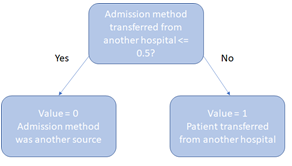
\includegraphics[width = 6cm]{Chapter4/Figures/ExampleDT.png}
%     \caption{Example Decision Tree Split}
%     \label{Fig:ExampleDT}
% \end{figure}
%The max number of end nodes was set to 20, to avoid over-fitting and reduce computational time, the number of minimum samples per leaf was set to 500.
Subsections \ref{sec:predcontLOS} and \ref{sec:predgroupLOS}, will now generate CART models based on continuous LOS and grouped LOS.
\subsection{Predicting Continuous LOS}\label{sec:predcontLOS}
The LOS of a patient is important for resource planning and the hospital requirements for the patients. As shown within Table \ref{Tab:ContinuousLOS-Lin}, the variable `No. of Scans' resulted in a larger R$^2$ value than `Scan Y/N', and as a result, moving forward this variable will be used within the the CART tree. Similarly, `Diagnosis' had a larger R$^2$ value than the `ICD10 - First Letter', so diagnosis will be the variable included in the analysis. The variables age and frailty will be considered both continuously and categorically. 

Regression trees will be coded within python using X package and the mean squared error. The mean square error determines where splits should occur by calculating how much the prediction deviated from the original target.
\begin{equation}\label{eq:MSE}
    \text{MSE} = \frac{1}{n}\sum^{n}_{i=1}(Y_{i} - \hat{Y}_{i})^2
\end{equation}
where $Y$ is the actual value and $\hat{Y}$ is the prediction.

The model is scored using the accuracy... 
\begin{equation}
    Equation here?
\end{equation}

Parameter tuning? - Do i discuss? or just do?

\hl{Here should be the values in the code? - what did I mean}

There will be six combinations of different experiments performed to determine the highest accuracy combination. These combinations use continuous and grouped age, with no frailty, continuous frailty and grouped frailty categories.
\subsubsection{Continuous Age - Not Including Frailty}\label{Sec:Regression1}
\hl{from here}
Firstly, age was used as a continuous variable and the results produced an accuracy score of 0.3281. The results show us the most important factor in determining length of stay is whether a patients admission method was that they had arrived from another hospital. If the patient had, then the average LOS was 25.75 days. If the patient arrived via a different method then the average LOS was 4.75 days.
Further extending to change age to a grouped variable, the accuracy reduced to 0.3267, a decrease of 0.0014. Similar to the previous regression the first determining split was whether a patient was transferred from another hospital, however the overall Regression tree contains different splits.


\subsubsection{Including Continuous Frailty}\label{Sec:Regression2}
The frailty score was included as a continuous measure, as discussed in Section \ref{Sec:Frailty}. By adding frailty, the accuracy score was 0.3289, slightly higher than not including frailty at all. The difference within the regression trees can be seen within Figure \ref{Fig:Regsplit}, with a the split occurring on the specialty or the frailty score. The results also show a greater difference of LOS between the two groupings (149 hours compared to 37 hours).


\begin{figure}[h!]
\centering
\begin{subfigure}{.49\textwidth}
  \centering
  \captionsetup{justification=centering}
  \includegraphics[width=1\linewidth]{Chapter4/Figures/Split2.png}
  \caption{Section of Regression Tree,\\ No Frailty}
  \label{Fig:RegSplit1}
\end{subfigure}
\begin{subfigure}{.49\textwidth}
  \centering
  \captionsetup{justification=centering}
  \includegraphics[width=1\linewidth]{Chapter4/Figures/Split2a.png}
  \caption{Section of Regression Tree,\\ Continuous Frailty}
  \label{Fig:RegSplit2}
\end{subfigure}
\caption{Example Splits of the Regression Trees}
\label{Fig:Regsplit}
\end{figure}

Further, if age were to be grouped, then the accuracy reduces to 0.3272. One main difference if that the age is no longer included in the decision tree when it is included as a grouped measure. Within the two regression trees of continuous and grouped age, there are a number of different splits. Grouping age produces an accuracy score larger than if no including frailty, however when analysing frailty as a continuous measure, using continuous age produces a higher result.



\subsubsection{Including Grouped Frailty}\label{Sec:Regression3}
The regression tree produced an accuracy score of 0.3288. Within the tree, continuous age was included and the split fell on patients ages less than or 79 or greater than and equal to 79. Frailty group was also included in the final regression tree also. When analysing by grouped age, the score decreased by 0.0013. However, by grouping age the accuracy score did increase on other grouped age analysis, with a score of 0.3275. Within the regression tree, both frailty group and age group are included in the final tree, although the two trees contain splits in different places.

\subsubsection{Comparisons}
Amongst the regression analysis, the highest accuracy was calculated to be 0.3289 and was produced from using both age and frailty as a continuous measure (Figures \ref{fig:Cartsplit1}, \ref{fig:Cartsplit2}, and \ref{fig:Cartsplit3}).. The order of the splits can be seen within Appendix \ref{Sec:RegressionTreeCode}. 

All six accuracy scores fall between 0.3267 and 0.3281, showing that there is not much difference depending on which combination used. The regression trees however do show a difference in the splitting node variables. An accuracy of roughly 32\% is rather low, nevertheless this can be explained by the large range of continuous LOS within the data and by only having 20 end nodes. However, it does provide a start for analysing similar groups of patients.

\begin{table}[h!]
\begin{adjustwidth}{0cm}{}
\centering\scalebox{1}{
\begin{tabular}{ccc}
\toprule
{\textbf{Variable}} & Continuous Age & Grouped Age\\ \midrule
No Frailty & 0.3281 & 0.3267 \\
Continuous Frailty & 0.3289 & 0.3272 \\
Grouped Frailty & 0.3288 & 0.3275 \\
\bottomrule
\end{tabular}}
\caption{Continuous LOS Accuracy Results}
\label{Tab:ContinuousLOS}
\end{adjustwidth}
\end{table}

\begin{landscape}
\begin{figure}
    \centering
    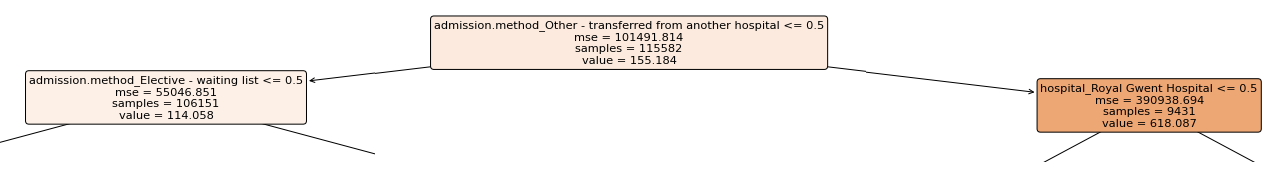
\includegraphics{Chapter4/Figures/Splitc.png}
    \caption{Regression Tree, first split}
    \label{fig:Cartsplit1}
\end{figure}

\begin{figure}
    \centering
    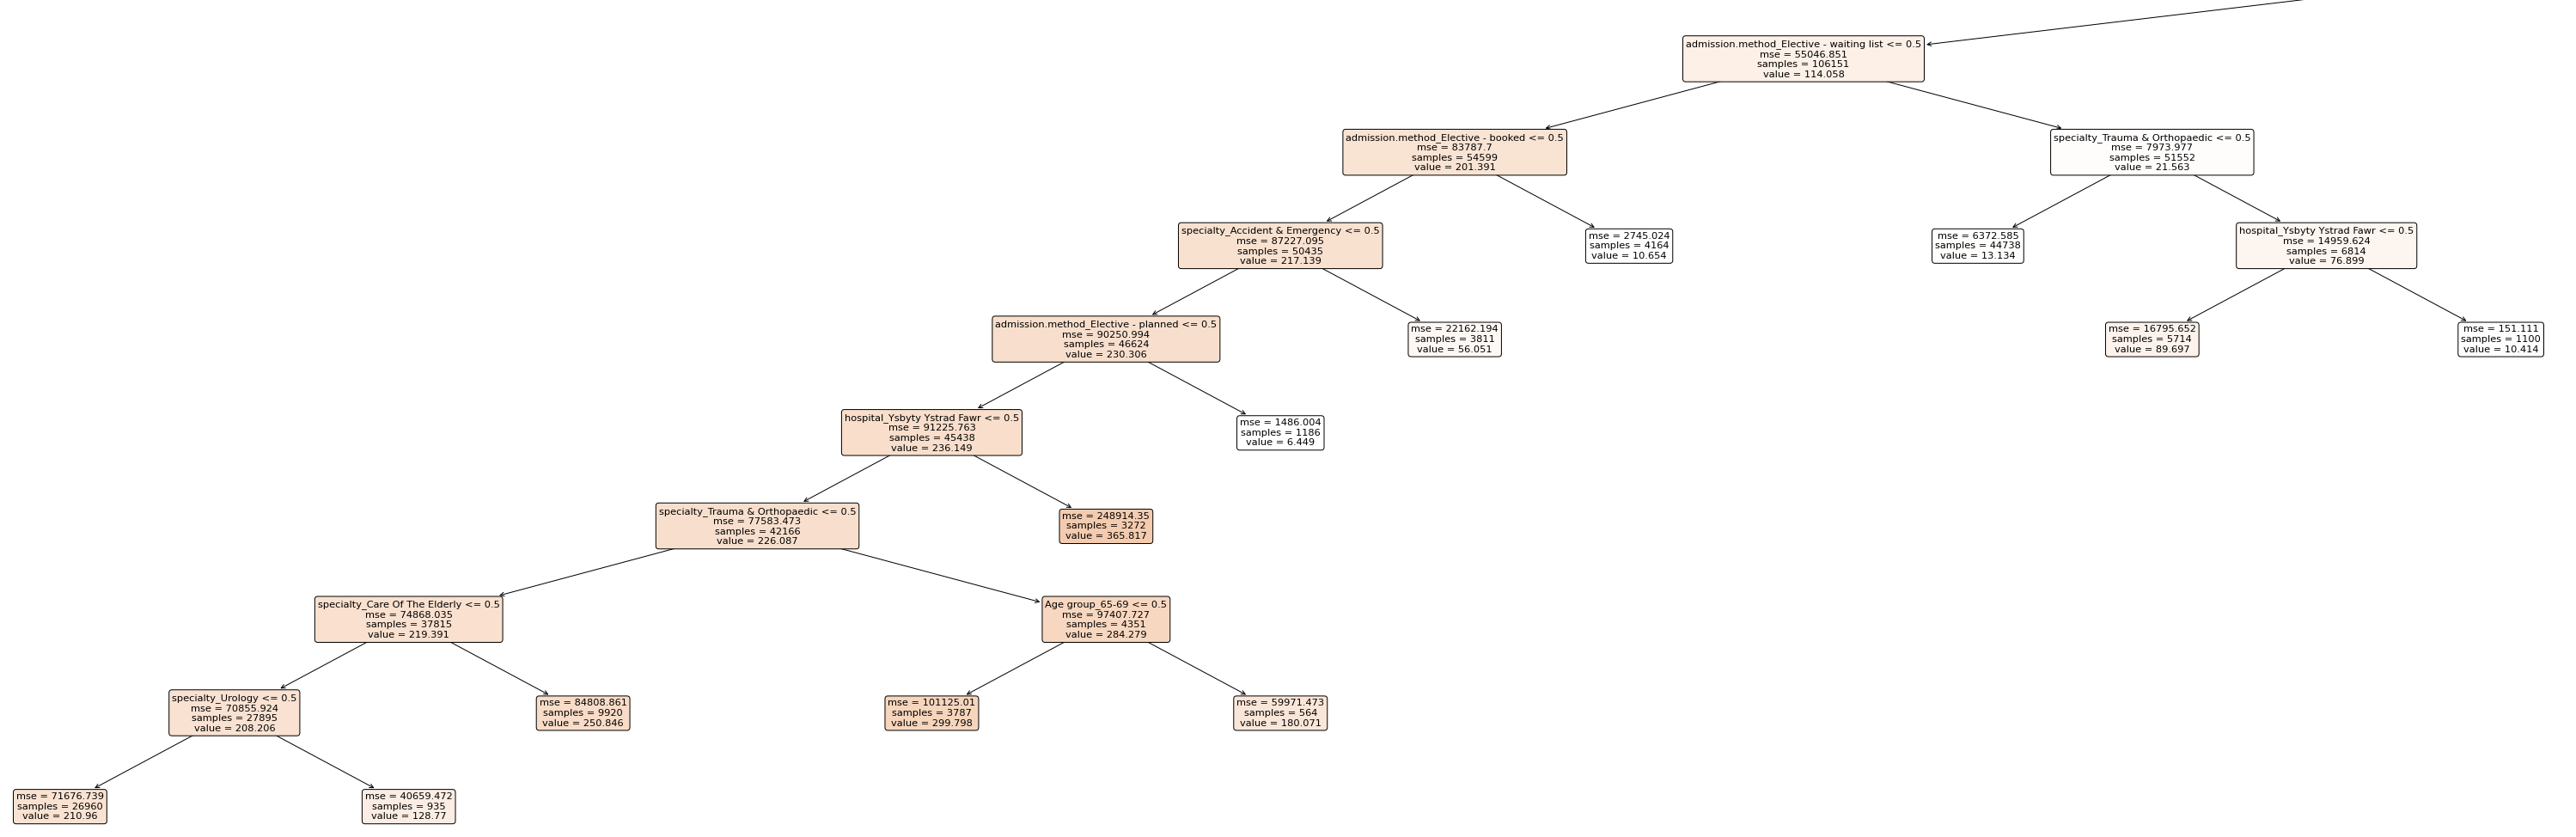
\includegraphics[width = 23cm]{Chapter4/Figures/Splita.png}
    \caption{Regression Tree, left split}
    \label{fig:Cartsplit2}
\end{figure}

\begin{figure}
    \centering
    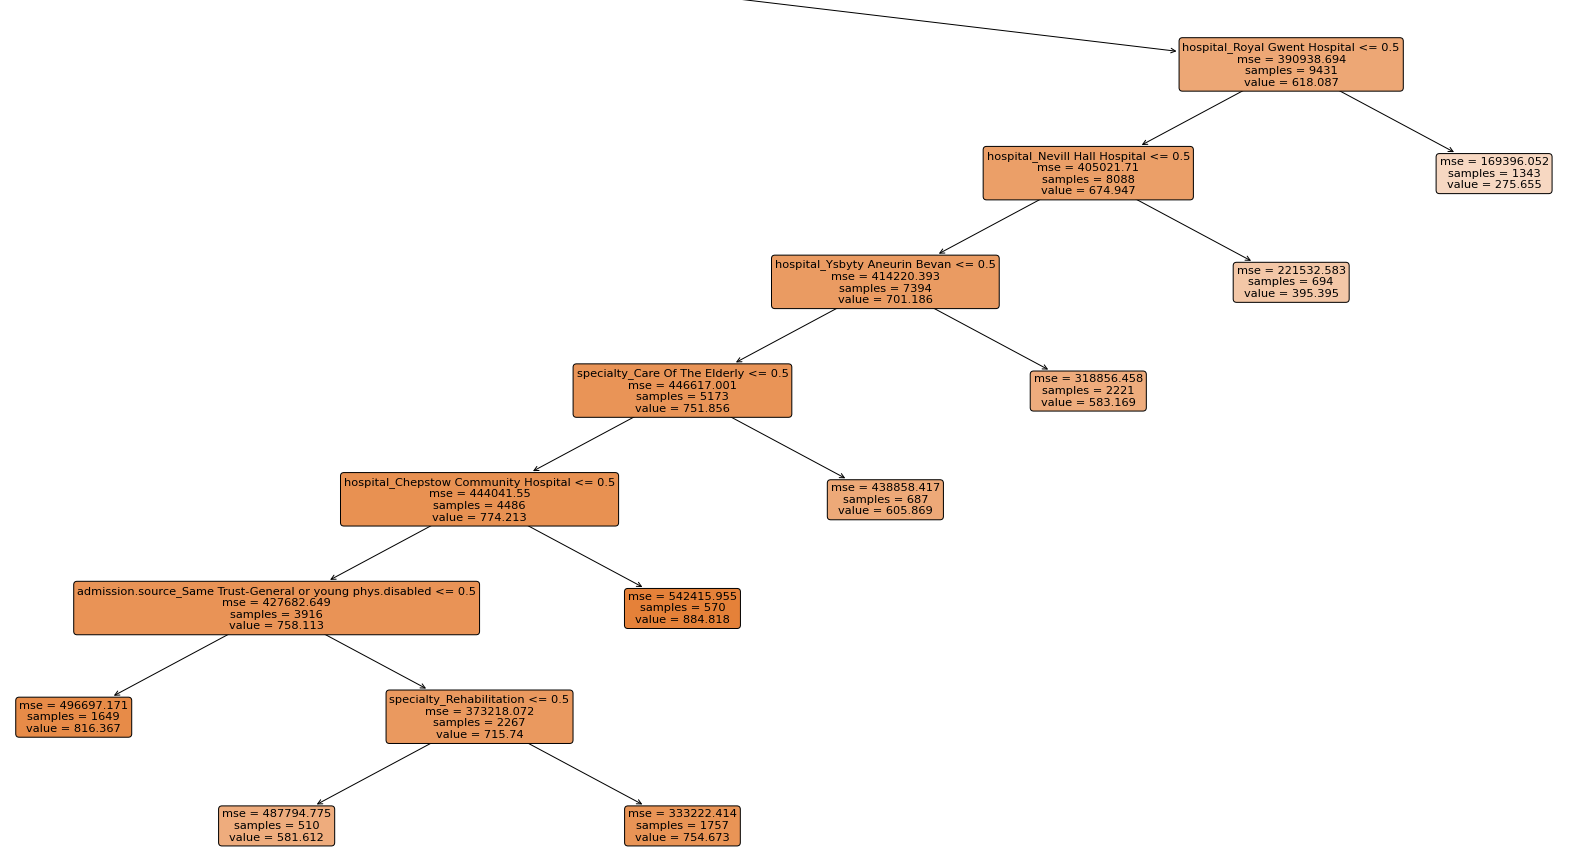
\includegraphics[width=23cm]{Chapter4/Figures/Splitb.png}
    \caption{Regression Tree, right split}
    \label{fig:Cartsplit3}
\end{figure}
\end{landscape}


\subsection{Predicting Grouped LOS}
The LOS of patients were then analysed by whether they were admitted overnight or discharged on the same day. Therefore, the two groups were `=0' or `$>$0' in their LOS. As a reminder, there were 75216 patients who fell into the `0 LOS' and 89902 patients who had a LOS greater than 0.

In order to determine where the best split occurs, the Gini index is calculated:
\begin{equation}
    \textrm{Gini index} = 1 - \sum^{n}_{i=1}p^{2}_{i}
\end{equation}
where i is the number of classes and $p_{i}$ is the probability of an object that is being classified to a particular class.

The Gini index is the sum of the square of the probabilities of each class and measures the inequality of the sample. It produces values between 0 and 1 and if a value of 0 is generated, it means the sample is perfectly homogeneous, i.e., all the elements are similar. A Gini index of 1 means maximal inequality among elements.

\subsubsection{Not Including Frailty}
The most determining factor as to whether a patient is likely to be admitted overnight when analysing with continuous age, is if the patient had the admission method of `Elective - waiting list'. An elective admission is a list of patients which a decision to admit has been made however  they are currently awaiting admission regardless of whether a date to admit has been given \cite{NHSDigital2021}. The accuracy score produced was calculated to be 0.8959, which is 0.5678 larger than the continuous LOS counterpart. Figure \ref{Fig:Confusion1a} demonstrates the confusion matrix, showing the number of patients falling into the true and predicted labels. By using age as a grouped variable the accuracy increases by 0.0029 to 0.8978. Analysing Figure \ref{Fig:Confusion1b}, it can be seen that there is an overall increase of 98 patients being correctly predicted. %The classification trees for continuous age and grouped age can be seen in Figure \ref{} and \ref{} respectively.

\begin{figure}[h!]
\centering
\begin{subfigure}{.5\textwidth}
  \centering
  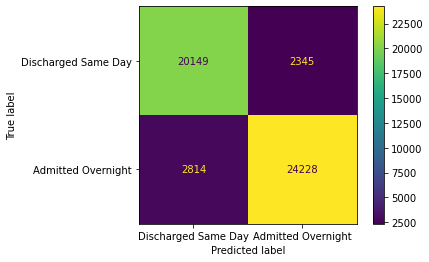
\includegraphics[width=1\linewidth]{Chapter4/Figures/FIG4AA.png}
  \caption{Continuous Age - No Frailty}
  \label{Fig:Confusion1a}
\end{subfigure}%
\begin{subfigure}{.5\textwidth}
  \centering
  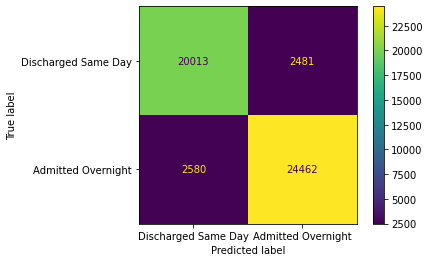
\includegraphics[width=1\linewidth]{Chapter4/Figures/FIG4BA.png}
  \caption{Grouped Age - No Frailty}
  \label{Fig:Confusion1b}
\end{subfigure}
\caption{Confusion Matrices - No Frailty}
\label{Fig:Confusion1}
\end{figure}

\subsubsection{Including Continuous Frailty}
By incorporating frailty into the CART analysis, the accuracy score remains at 0.8959, the same as the continuous age with no frailty included. Despite this, the classification tree is different, with a split occurring on whether frailty is less than 0.15 rather than if the hospital attended was Royal Gwent. By changing age from a continuous to a grouped measure, the classification tree goes unchanged and the accuracy score remains are 0.8959. Therefore, the confusion matrices displayed in Figure \ref{Fig:Confusion2} are identical.


\begin{figure}[h!]
\centering
\begin{subfigure}{.5\textwidth}
  \centering
  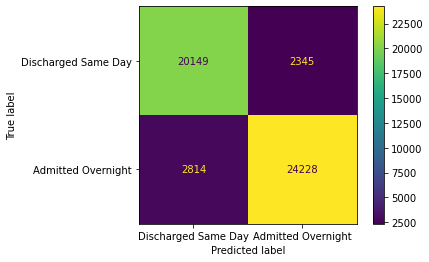
\includegraphics[width=1\linewidth]{Chapter4/Figures/FIG5AA.png}
  \caption{Continuous Age - Continuous Frailty}
  \label{Fig:Confusion2a}
\end{subfigure}%
\begin{subfigure}{.5\textwidth}
  \centering
  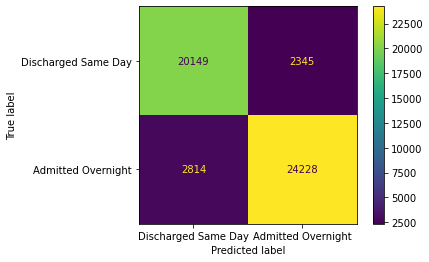
\includegraphics[width=1\linewidth]{Chapter4/Figures/FIG5BA.png}
  \caption{Grouped Age - Continuous Frailty}
  \label{Fig:Confusion2b}
\end{subfigure}
\caption{Confusion Matrices - Continuous Frailty}
\label{Fig:Confusion2}
\end{figure}

\subsubsection{Including Grouped Frailty}
The final CART analysis, included frailty as a grouped measure. The accuracy score again was found to be 0.8959, showing that there is no difference in accuracy when comparing across continuous age. There is a slight difference in the classification trees, with Figure \ref{Fig:CARTSsplit}, demonstrating the two different nodes from continuous frailty and grouped frailty.
\begin{figure}[h!]
\centering
\begin{subfigure}{.49\textwidth}
  \centering
  \captionsetup{justification=centering}
  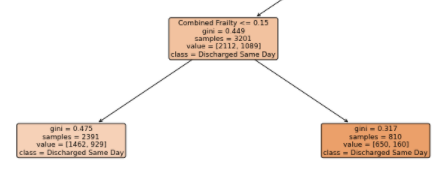
\includegraphics[width=1\linewidth]{Chapter4/Figures/Split1a.png}
  \caption{Section of CART Tree\\ Continuous Frailty}
  \label{Fig:CARTSplit1}
\end{subfigure}
\begin{subfigure}{.49\textwidth}
  \centering
  \captionsetup{justification=centering}
  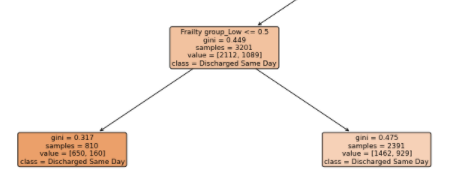
\includegraphics[width=1\linewidth]{Chapter4/Figures/Split1.png}
  \caption{Section of CART Tree, Figures \ref{fig:Class1}, \ref{fig:Class2}, \ref{fig:Class3}, \ref{fig:Class4},\\ Grouped Frailty}
  \label{Fig:CARTSplit2}
\end{subfigure}
\caption{Example Splits of the CART Trees}
\label{Fig:CARTSsplit}
\end{figure}

Similarly, changing to grouped age rather than continuous age, produces the same accuracy score of 0.8959.


\subsubsection{Comparisons}
Table \ref{Tab:GroupedLOS} provides an overview of the classification trees and the associated accuracy scores. All six accuracy scores are greater than 89\%. The highest accuracy score originates from the grouped age and no frailty combination (See Figures \ref{fig:Class1}, \ref{fig:Class2}, \ref{fig:Class3}, \ref{fig:Class4}). The remaining five all have the same accuracy score, however they have slightly different classification tree structures.

\begin{table}[h!]
\begin{adjustwidth}{0cm}{}
\centering\scalebox{1}{
\begin{tabular}{ccc}
\toprule
{\textbf{Variable}} & Continuous Age & Grouped Age\\ \midrule
No Frailty & 0.8959 & 0.8978 \\
Continuous Frailty & 0.8959 & 0.8959 \\
Grouped Frailty & 0.8959 & 0.8959 \\
\bottomrule
\end{tabular}}
\caption{Grouped LOS Accuracy Results}
\label{Tab:GroupedLOS}
\end{adjustwidth}
\end{table}

\begin{landscape}
\begin{figure}
    \centering
    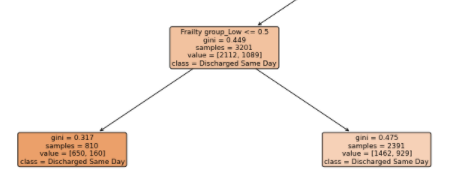
\includegraphics[scale =0.8]{Chapter4/Figures/Split1.png}
    \caption{Classification Tree, first split}
    \label{fig:Class1}
\end{figure}

\begin{figure}
    \centering
    \includegraphics[scale =0.8]{Chapter4/Figures/Split2.png}
    \caption{Classification Tree, left split}
    \label{fig:Class2}
\end{figure}

\begin{figure}
    \centering
    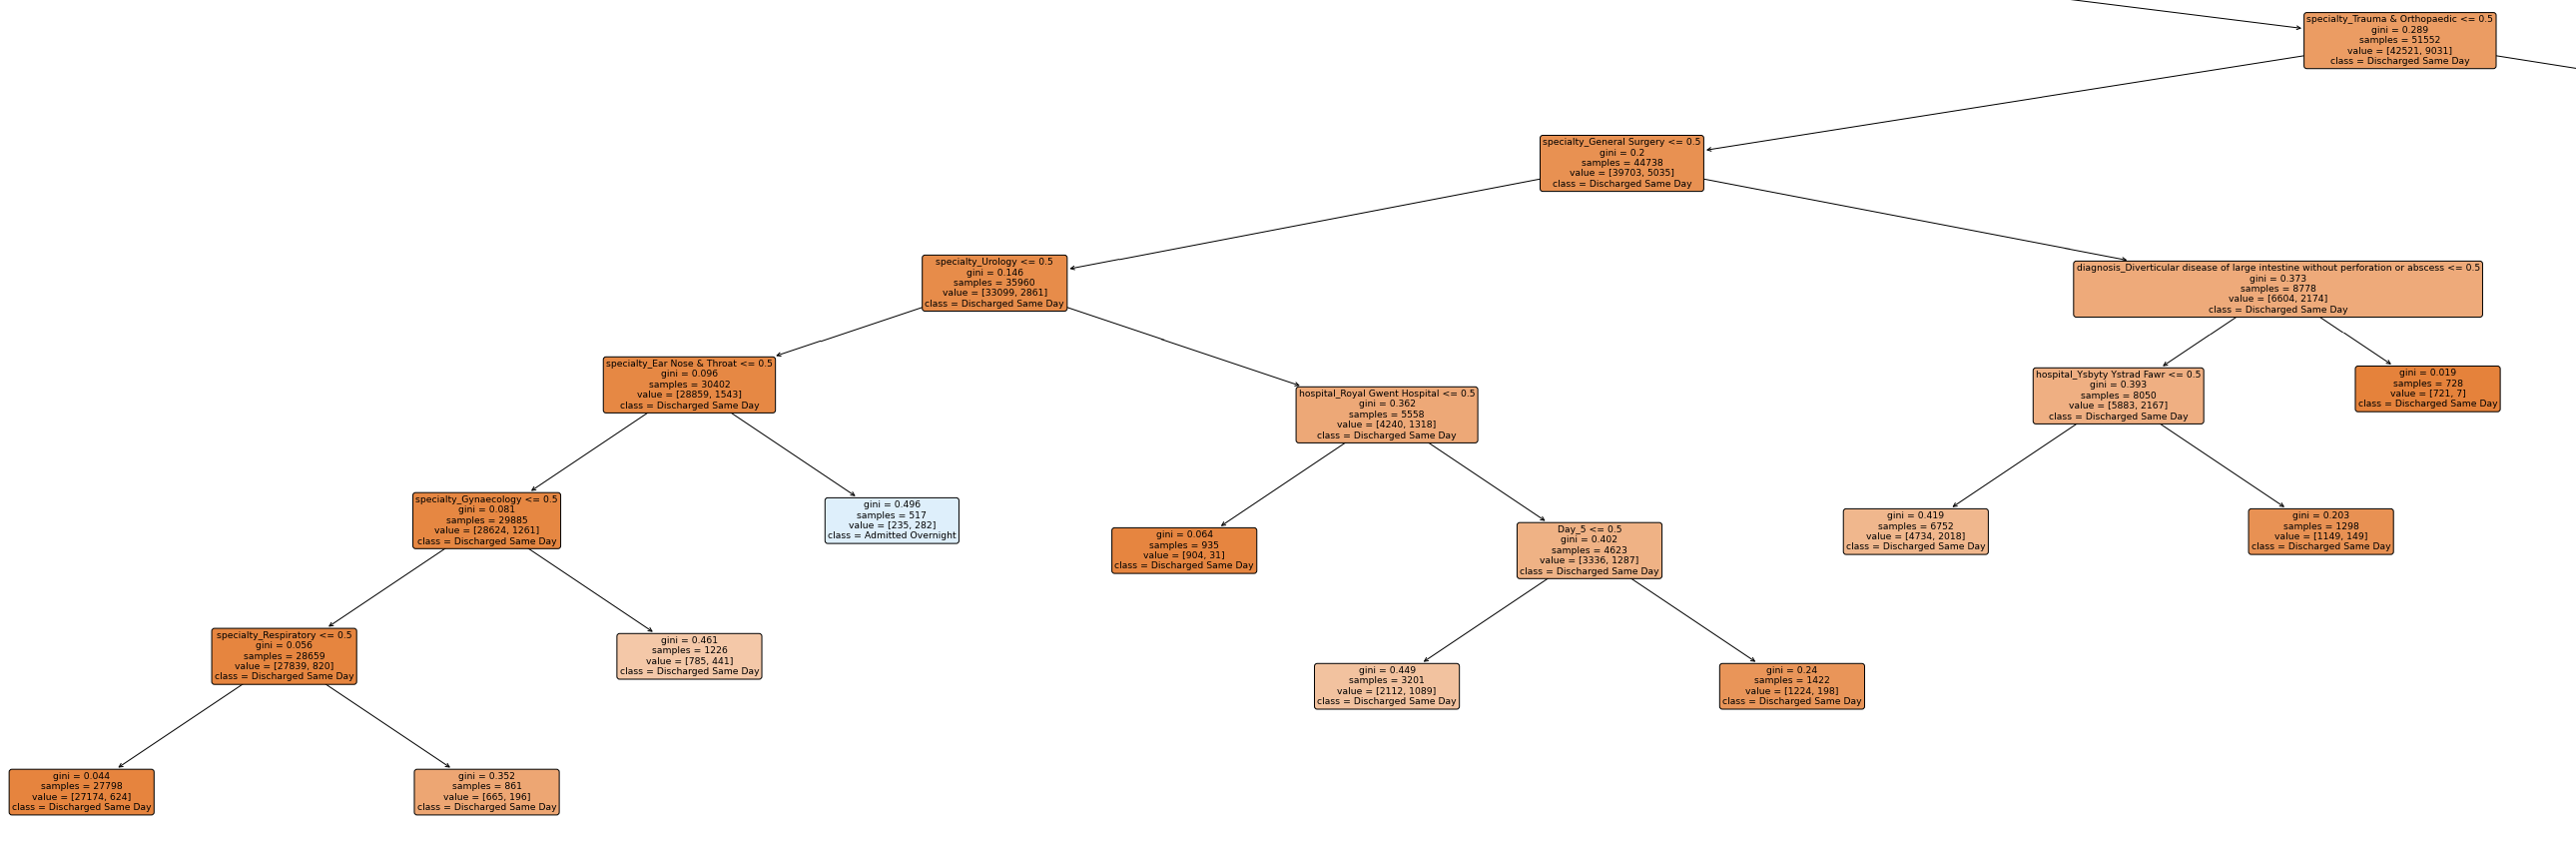
\includegraphics[scale =0.5]{Chapter4/Figures/Split3.png}
    \caption{Classification Tree, right split, then left split}
    \label{fig:Class3}
\end{figure}
\begin{figure}
    \centering
    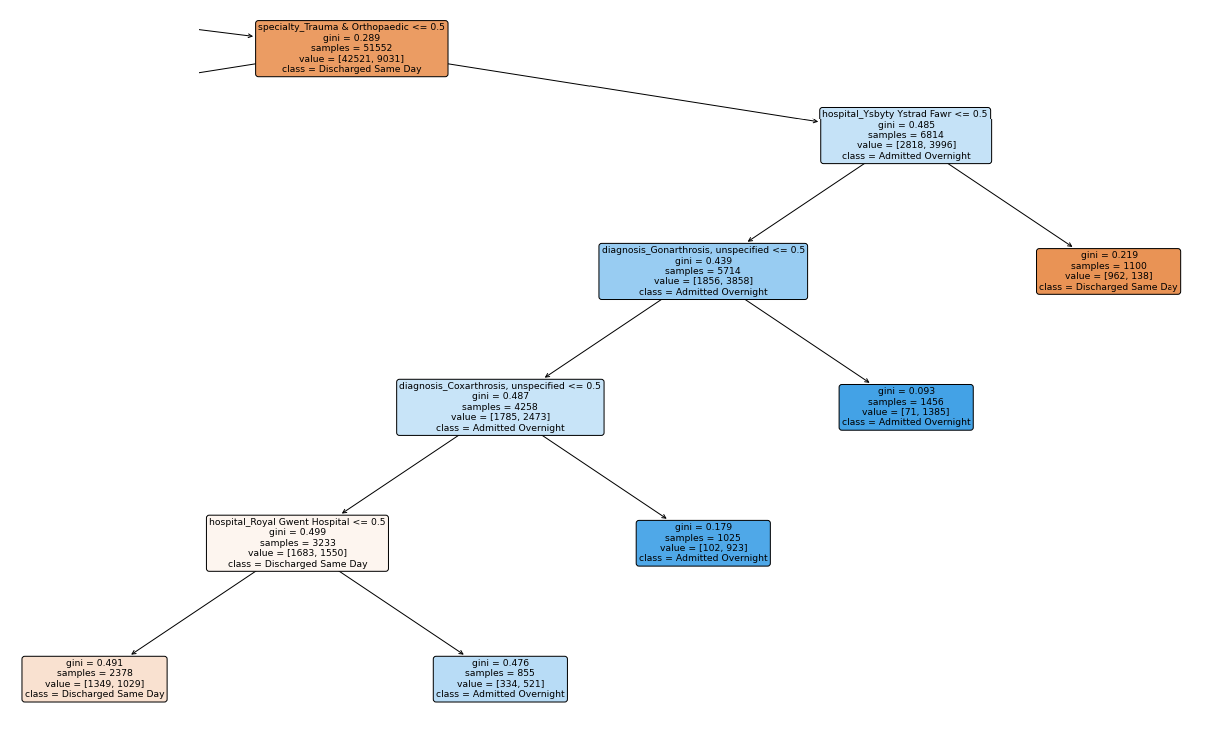
\includegraphics[scale=0.8]{Chapter4/Figures/Split4.png}
    \caption{Classification Tree, right split, then right split}
    \label{fig:Class4}
\end{figure}
\end{landscape}

If the minimum number of samples per leaf was not set to 500, the maximum accuracy score would increase to 0.8989. This is only an increase of 0.0021 on the highest scoring results from Table \ref{Tab:GroupedLOS}, however, it results in smaller samples being present in the leaves, i.e., 257 and 312 patients (Figures \ref{Fig:Split1} and \ref{Fig:Split2}).

\begin{figure}[h!]
\centering
\begin{minipage}{.5\textwidth}
  \centering
  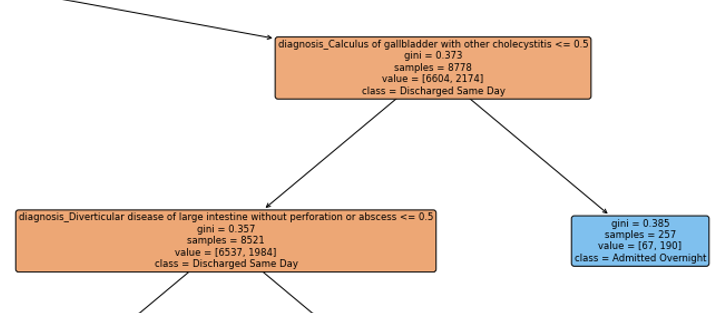
\includegraphics[width=1\linewidth]{Chapter4/Figures/FIGX1a.png}
  \captionof{figure}{Sample split of 257}
  \label{Fig:Split1}
\end{minipage}%
\begin{minipage}{.5\textwidth}
  \centering
  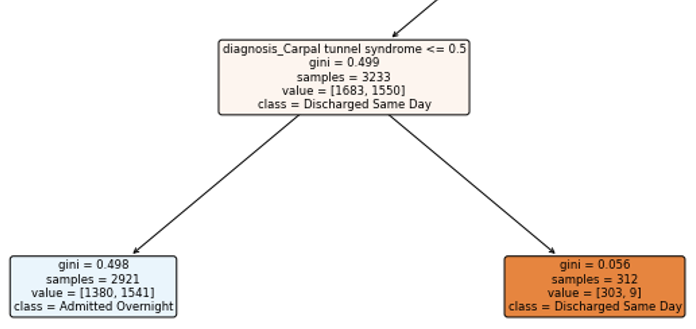
\includegraphics[width=0.9\linewidth]{Chapter4/Figures/FIGX1b.png}
  \captionof{figure}{Sample split of 312}
  \label{Fig:Split2}
\end{minipage}
\end{figure}

\subsection{Comparisons between Continuous and Grouped LOS Prediction}
For all cases, grouping LOS increases the accuracy scores by at least 56\% (Table \ref{Tab:CombinedCART}). The highest accuracy score for LOS depends on the combination of elements. If analysing continuous LOS, then the highest accuracy is produced by continuous age and frailty with 0.3289. However, with no frailty present and a grouped aged variable produced the highest accuracy score for grouped LOS. 

\begin{table}[h!]
\centering\scalebox{1}{
\begin{tabular}{ccccc}
\toprule
\multirow{2}{*}{\textbf{Variable}} & \multicolumn{2}{c}{\textbf{Continuous LOS}} &  \multicolumn{2}{c}{\textbf{Grouped LOS}}  \\ %\cline{3-5}
&\textbf{Continuous Age}& \textbf{Grouped Age}& \textbf{Continuous Age} & \textbf{Grouped Age}\\ \midrule
\textbf{No Frailty} & 0.3281 &0.3267 &0.8959 & 0.8978 \\
\textbf{Continuous Frailty} & 0.3289 & 0.3272 & 0.8959 &0.8959 \\
\textbf{Grouped Frailty} & 0.3288 &0.3275 & 0.8959 &0.8959 \\\bottomrule
\end{tabular}}
\caption{Combined CART Results}
\label{Tab:CombinedCART}

\end{table}

%\hl{Add some more here}

%\hl{If have time look at multiple groups - at least for one of the categories? Early on in the code - already coded :)}

\subsection{Predicting Spell Patients}
Within the data there were 9,464 patients who were part of a spell. This meant they were discharged from hospital and readmitted to the same hospital or one within ABUHB on the same day. Patients who were in a spell had their first hospital frailty score for the entire stay summed, meaning the range in frailty scores increased to 10.4. The decision trees have been run using a maximum of 15 leaf nodes.

\subsubsection{No Including Frailty}
The accuracy was considerably high with a result of 0.9386, however after further inspection of the confusion matrix (Figure \ref{Fig:CM1}, it can be seen that all patients are being predicted as single spells, and therefore it is assuming that no patient will have a spell. This is most likely due to the small proportion of patients which fall into the spell category.
\begin{figure}[h!]
    \centering
    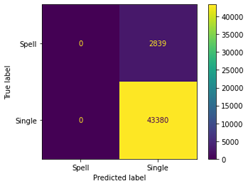
\includegraphics[width = 6cm]{Chapter4/Figures/Matrix1.png}
    \caption{Spell Confusion Matrix - No Frailty}
    \label{Fig:CM1}
\end{figure}

\subsubsection{Including Continuous Frailty}
The accuracy for continuous frailty was calculated to be 0.9429, an increase of 0.0043. The confusion matrix shows that by adding frailty 205 Spell patients were correctly predicted and therefore by including continuous frailty shows an improvement in prediction ability (Figure \ref{Fig:CM2}). 
\begin{figure}[h!]
    \centering
    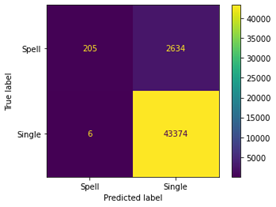
\includegraphics[width = 6cm]{Chapter4/Figures/Matrix2.png}
    \caption{Spell Confusion Matrix - Continuous Frailty}
    \label{Fig:CM2}
\end{figure}
\subsection{Comparisons}
Figures \ref{Fig:CM1} and \ref{Fig:CM2} show the difficulty in prediction of Spell patients, with the given parameters. If more patients were part of a spell, then there would be a higher quantity of patients to train the model on, however only 5.73\% of patients were part of a spell. 


\end{document}
